

\documentclass[color=usenames,dvipsnames]{beamer}

\usepackage[adobefonts,noindent]{ctex} %中文支持
\setCJKmainfont{SimSun}

\mode<presentation> {

\usetheme{Madrid}
\usecolortheme{lily}
\useoutertheme{infolines}

}


\usepackage{booktabs} 
\usepackage{tikz}


% Thin fonts
\usepackage{cmbright}
\usepackage[T1]{fontenc}

% 为了插入c代码
\usepackage{listings}
\usepackage{fontspec}
\newcommand{\cCode}[0]{\lstset{language=C++,
                basicstyle=\ttfamily,
                keywordstyle=\color{blue}\ttfamily,
                stringstyle=\color{red}\ttfamily,
                commentstyle=\color{OliveGreen}\ttfamily,
                morecomment=[l][\color{magenta}]{\#}
}}
\newfontfamily\listingsfont[Scale=.7]{SimSun}
\lstset{frame=single}


\newcommand{\setof}[1]{\ensuremath{\left \{ #1 \right \}}}
\newcommand{\tuple}[1]{\ensuremath{\left \langle #1 \right \rangle }}
\newcommand{\red}[1]{\textcolor{red}{#1}}
\newcommand{\brown}[1]{\textcolor{brown}{#1}}
\newcommand{\green}[1]{\textcolor{green}{#1}}
\newcommand{\blue}[1]{\textcolor{blue}{#1}}
\newcommand{\cyan}[1]{\textcolor{cyan}{#1}}
\definecolor{dark_grey}{gray}{0.5}
\setbeamercolor{normal text}{fg=dark_grey,bg=white}
\setbeamertemplate{navigation symbols}{}

\setbeamercolor*{palette primary}{fg=gray!100,bg=gray!10}
\setbeamercolor*{palette quaternary}{fg=gray!100,bg=gray!10}
\setbeamercolor*{palette secondary}{fg=gray!100,bg=gray!20}
\setbeamercolor*{palette tertiary}{fg=gray!100,bg=gray!10}
\setbeamercolor*{navigation symbols}{fg=white,bg=white}
\usefonttheme{default}


\setbeamertemplate{blocks}[rounded][shadow=false]
\setbeamercolor{block title}{bg=gray!10}
\setbeamercolor{block body}{fg=gray,bg=gray!10}
%\setbeamercolor{frametitle}{fg=}

\setbeamertemplate{frametitle}[default][center]

\setbeamertemplate{itemize items}[default]
\setbeamertemplate{enumerate items}[default]

\newcommand{\F}{\mathbb{F}}

%  动态调节长度的 block
\usepackage[customcolors,shadow,roundedcorners]{dynblocks}
\usepackage{environ}
\newsavebox\mybox
\NewEnviron{cdyn}[1]{%
    \sbox{\mybox}{$\BODY$}%
    \begin{center}
    \begin{dynblock}
    \opaqueblock<#1>[\wd\mybox]{\[\BODY\]}
    \end{dynblock}
    \end{center}
}{}%

\title[COE2015上机题]{计算概论习题课}
\subsection{上机模拟,结构体指针,综合练习}
\author{韩喆}
\institute{WIP@ICST}
\date{20151221}
\begin{document}


\begin{frame}
  \titlepage
\end{frame}

% Uncomment these lines for an automatically generated outline.
%\begin{frame}{Outline}
%  \tableofcontents
%\end{frame}

\section{简介}

\begin{frame}{简介}\footnotesize

\begin{columns}
 \column{0.45\hsize}
讲最近三次上机内容
\vspace{0.5cm}

 \begin{block}{综合练习}
\sout{转输出矩阵} \\ 
例题(7.6) 不能一起吃的食物 \\ 
例题(15.5) 算24 (1103) \\ 
进制转换 \\ 
\sout{计算反序数} \\ 
\sout{放苹果问题} \\ 
\sout{习题(14-3) 奇数单增序列} \\ 
\sout{1090 分解因数} \\ 
习题(15-1) 前缀表达式 (1010) \\ 
\sout{文字排版} \\ 
\sout{验证子串 }
 \end{block}
 

 \column{0.45\hsize}
 \begin{block}{结构体与链表}
 删除数组中的元素(链表)\\ 
统计学生信息(使用动态链表完成)\\ 
\sout{谁拿了最多奖学金}\\ 
班级学生成绩统分\\ 
链表合并排序
 \end{block}
 \begin{block}{模拟}
 满足条件的数累加\\ 
字母次数\\ 
\sout{求均方差(用指针完成)}\\ 
提取数字串按数值排序\\ 
二维数组回形遍历\\ 
扩号匹配问题\\ 
连续整数区域上确界
 \end{block} 
\end{columns}

\end{frame}

\section{期末上机模拟}


\frame{
  \begin{columns}[c]
   \column{.15\hsize}
   \column{.7\hsize}
   \begin{block}{}
    \centering \Large 期末上机模拟  \\ 
    \small --- 1214
   \end{block}
   \column{.15\hsize}
  \end{columns}
}

\subsection{1.满足条件的数累加}
\frame{
  \frametitle{满足条件的数累加}
    \begin{columns}
     \column{0.5\hsize}
     \only<1>{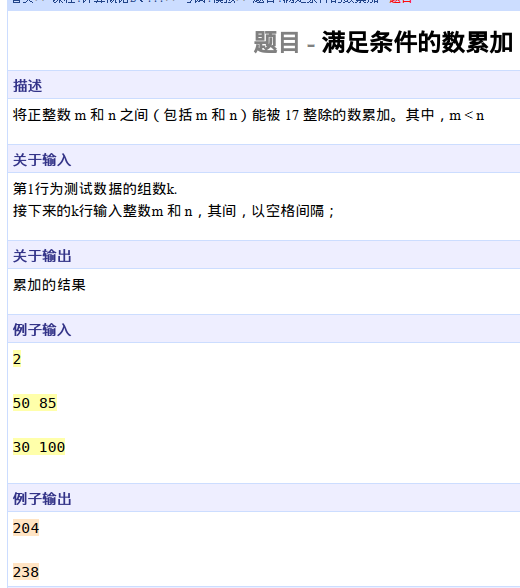
\includegraphics[width=0.9\hsize]{pic/满足条件的数累加.png}}
     \only<2>{
      \begin{itemize}
       \item 注意利用VS的自动排版
       \item 不需要数组存储,来一个$m,n$,处理一个$m,n$就好
      \end{itemize}
      }
     
     \column{0.5\hsize}
    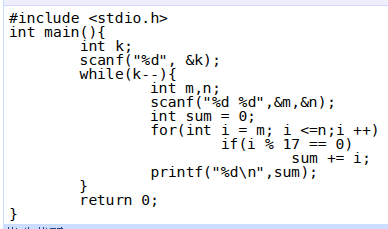
\includegraphics[width=0.9\hsize]{pic/满足条件的数累加-good.png} \\
    \vspace{0.1cm}
    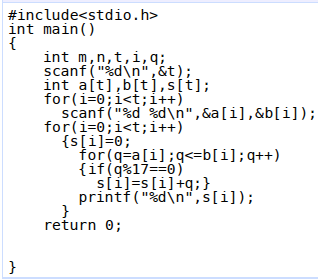
\includegraphics[width=0.8\hsize]{pic/满足条件的数累加-bad.png}
    \end{columns}
}

\subsection{2.字母次数}
\frame{
  \frametitle{字母次数}
     \only<1-2>{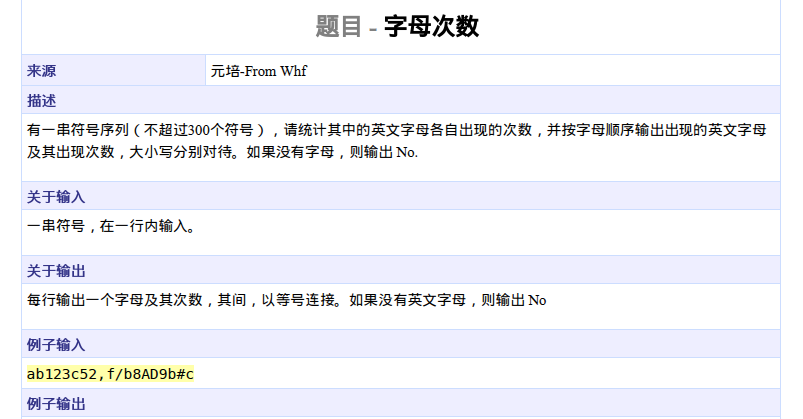
\includegraphics[width=0.9\hsize]{pic/字母次数-o.png}
     \only<2>{
      \begin{itemize}
       \item 如何判断字符等价?判读字符在某个范围?
      \end{itemize}
      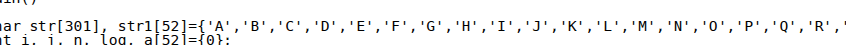
\includegraphics[width=0.99\hsize]{pic/字母次数-bad2.png}\\ 
      }
      }
      \only<3>{
    \begin{columns}
     \column{0.7\hsize}
     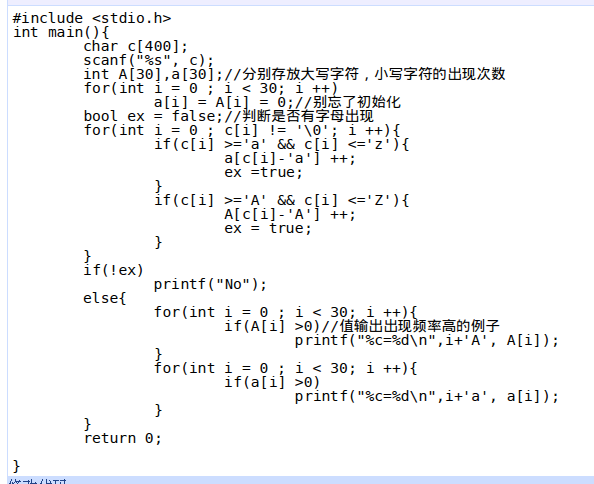
\includegraphics[width=1\hsize]{pic/字母次数.png}
     \column{0.3\hsize}
     \begin{itemize}\footnotesize
      \item A[1]=A['B'-'A']表示'B'的出现次数
      \item a[3]=A['d'-'a']表示'd'的出现次数
     \end{itemize}
    \end{columns}
     }
     
}

\subsection{3.求均方差(用指针完成)}
\frame{
  \frametitle{求均方差(用指针完成)}
     \only<1>{\centering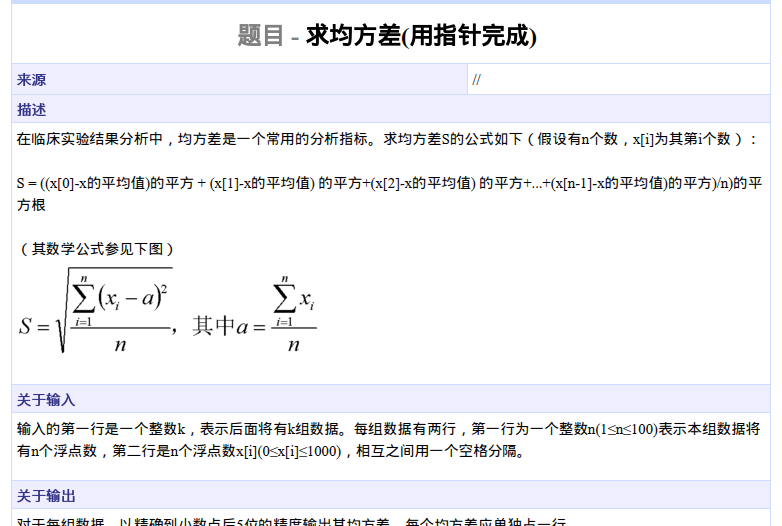
\includegraphics[width=0.8\hsize]{pic/均方误差.png}}
     \only<2>{
     \begin{columns}
      \column{0.35\hsize}
     \begin{itemize}
      \item 读取用指针
     \end{itemize}
     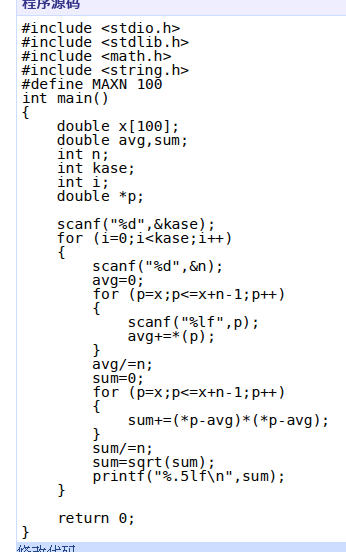
\includegraphics[width=0.95\hsize]{pic/均方误差-good2.png}
     
     \column{0.6\hsize}
     \begin{itemize}
      \item 指针+结构体
     \end{itemize}
     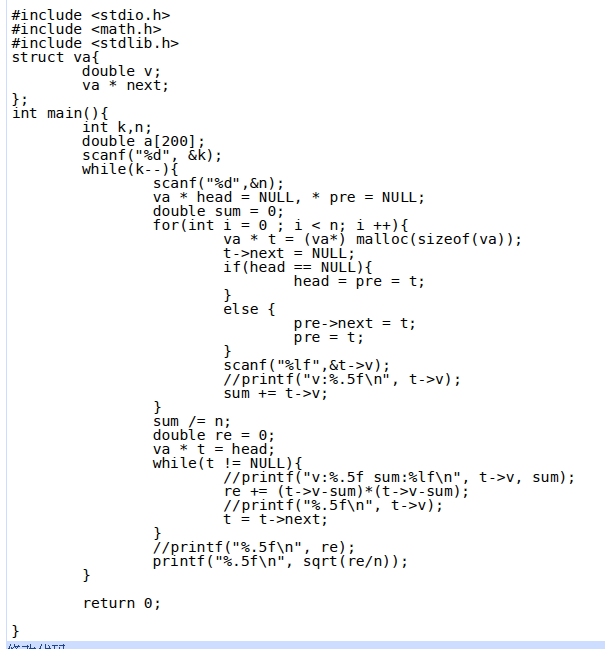
\includegraphics[width=0.99\hsize]{pic/均方误差-good.png}
     \end{columns}
     }
}

\subsection{4.提取数字串按数值排序}
\frame{
  \frametitle{提取数字串按数值排序}
     \only<1>{\centering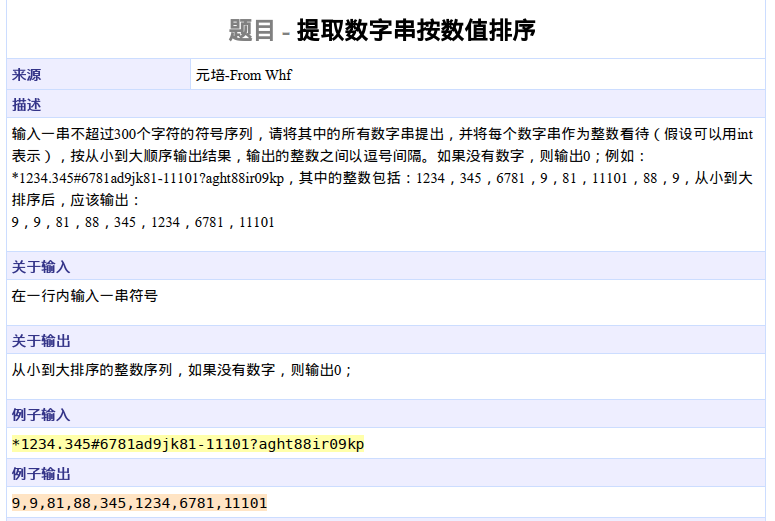
\includegraphics[width=0.9\hsize]{pic/提取数字串按数值排序.png}}
     \only<2>{
     \begin{columns}
      \column{0.35\hsize}	
     \begin{itemize}
      \item 一个指针顺序扫每个字符
      \item 一个变量保存当前的数字大小(小于0表示没有数字)
      \item 扫到数字之后的下一个字符时把刚刚存储的数字加入数组,并把变量置为-1
      \item 最后对数组排序
     \end{itemize}
     
     \column{0.6\hsize}
     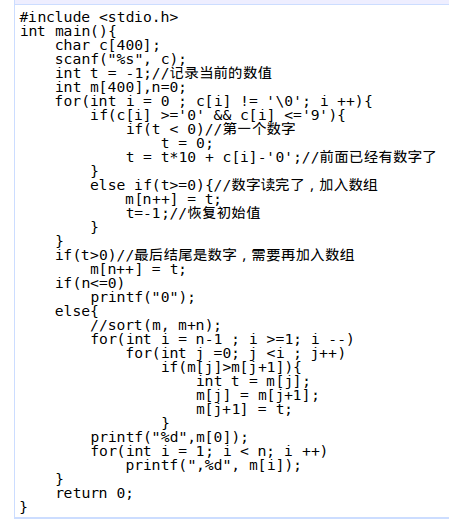
\includegraphics[width=0.9\hsize]{pic/提取数字串按数值排序-good.png}
     \end{columns}
     }
     \only<3>{
     \begin{columns}
      \column{0.35\hsize}	
     \begin{itemize}\footnotesize
      \item 这是我随便找的\textbf{没有过的例子}
      \item 这个同学至少犯了以下\textbf{错误}
     \end{itemize}
     \begin{enumerate}\footnotesize
      \item 数组开的不够大(至少\textbf{301},建议\red{330}+)
      \item 数组a\red{没有初始化}
      \item \red{字符和整数}的关系没有搞明白
	\begin{itemize}\footnotesize
	 \item 'c'-'a'=2
	 \item 'a'-2=95
	 \item str[i] = '0'=48
	\end{itemize}
     \item $a[j+1]=a[j]*10+...$ 两者实际上没关系,这个式子肯定有问题
     \item 输出是a[0]还是a[1]开始?

     \end{enumerate}

     
     \column{0.6\hsize}
     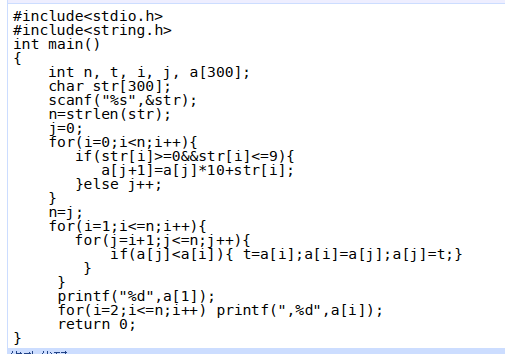
\includegraphics[width=0.9\hsize]{pic/提取数字串按数值排序-bad.png}
     \end{columns}
     }
}

\subsection{5.二维数组回形遍历}
\frame{
  \frametitle{5.二维数组回形遍历}
  
     \only<1>{\centering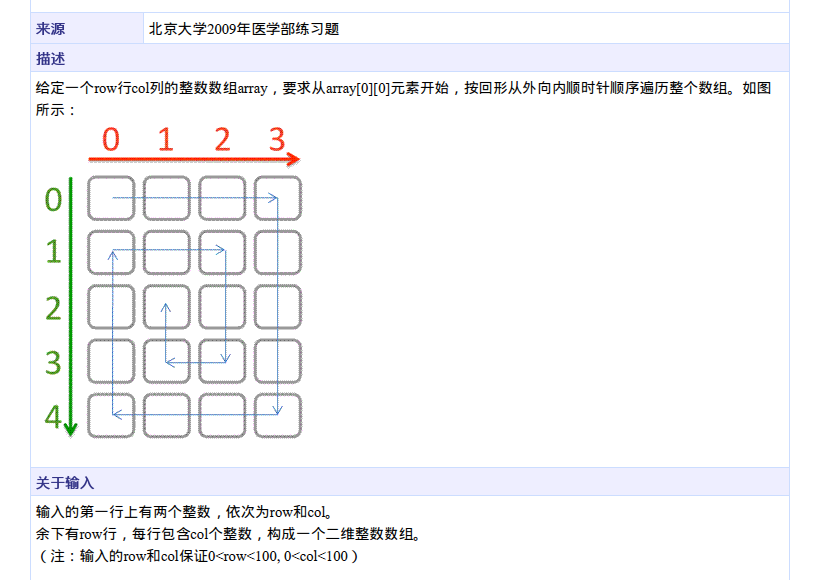
\includegraphics[width=0.9\hsize]{pic/二维数组回形遍历.png}}
     \only<2>{
     \begin{columns}
      \column{0.35\hsize}	
     \begin{itemize}
      \item 每次从左上角开始顺时针扫描一圈
      \item 移动起始点,继续做
      \item \blue{考虑清楚结束条件}
      \item 考虑清楚每圈的行坐标,列坐标
     \end{itemize}
     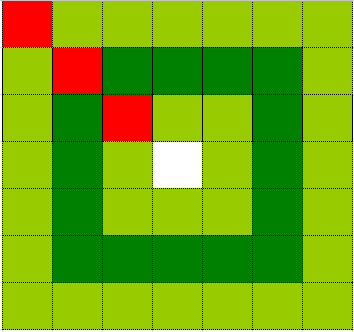
\includegraphics[width=0.9\hsize]{pic/二维数组回形遍历-思路1.png}
     
     
     \column{0.6\hsize}
     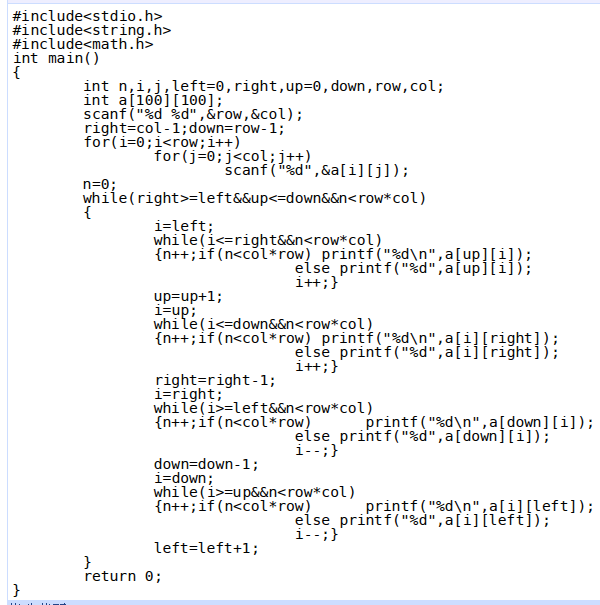
\includegraphics[width=0.9\hsize]{pic/二维数组回形遍历-good1.png}
     \end{columns}
     }
     
     \only<3>{
     \begin{columns}
      \column{0.4\hsize}	
     \begin{itemize}\footnotesize
      \item 模拟真实行走过程
      \item 开始位置+方向
      \item 如果改方向下一个格子不在棋盘内或者下一个格子走过了,改变方向
      \item 如何改变方向?(下一个方向是?)
	\begin{itemize}\footnotesize
	 \item $(0,1)->(1,0)->(0,-1)->(-1,0)->(0,1)$
	\end{itemize}

      \item 判断在棋盘内且没有走过?
      \item 停止条件?
      \item \red{全局变量}:函数共用
     \end{itemize}
     
     \column{0.55\hsize}
     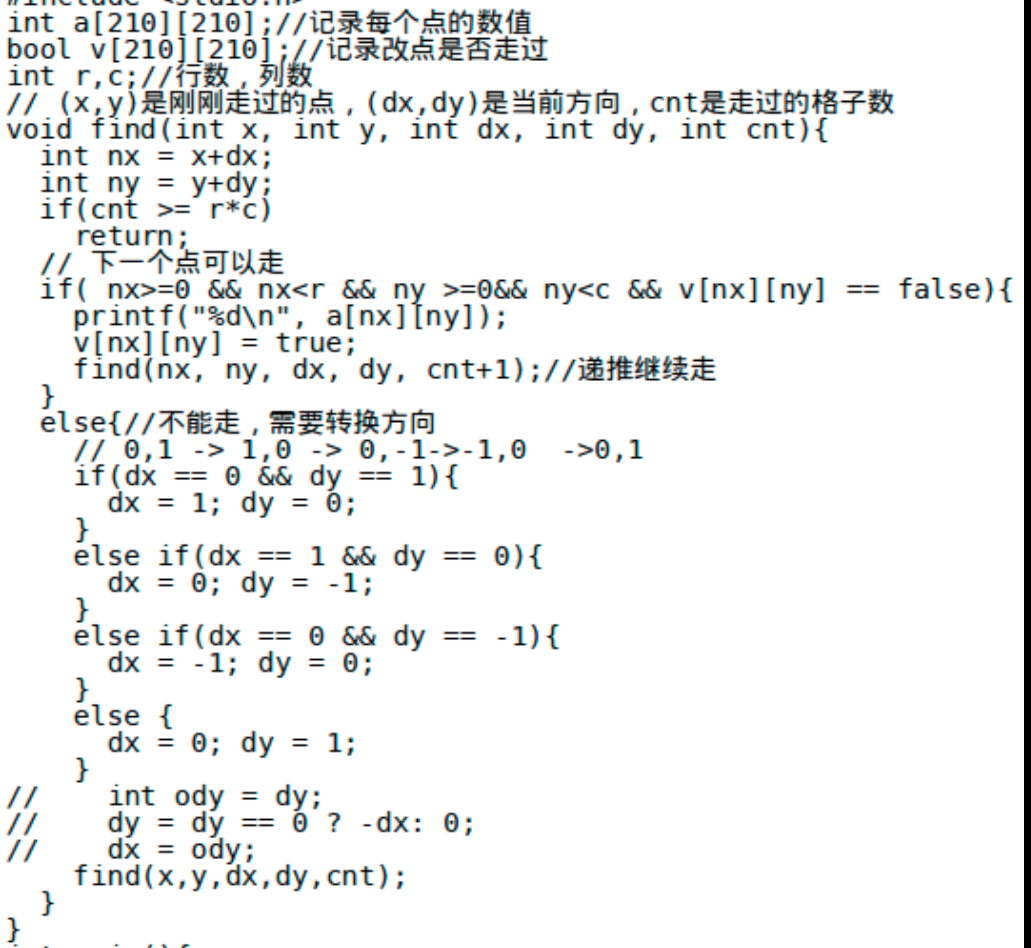
\includegraphics[width=0.9\hsize]{pic/二维数组回形遍历-good2.png}
     \end{columns}
     }
}



\subsection{6.扩号匹配问题}
\frame{
  \frametitle{6.扩号匹配问题}
  
     \only<1>{\centering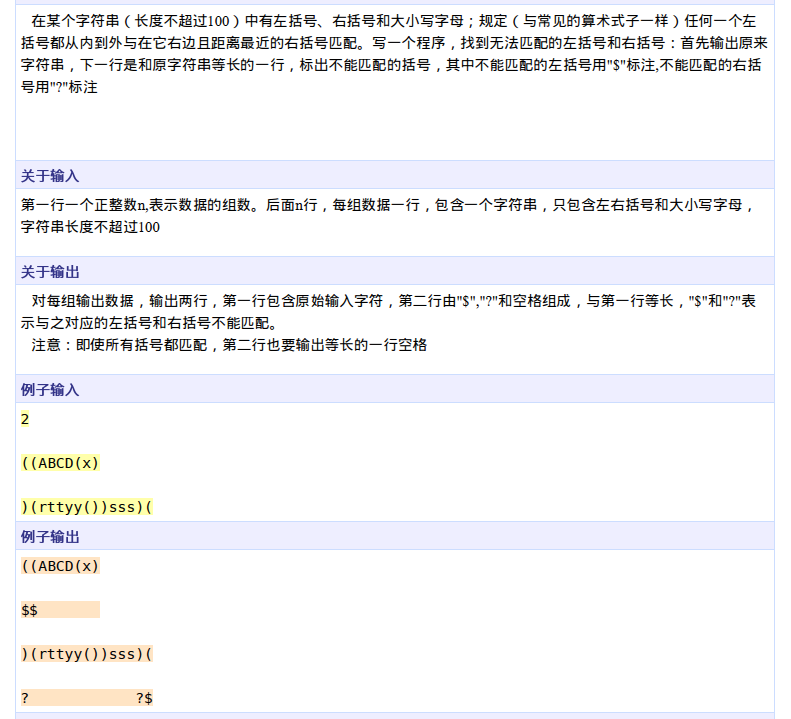
\includegraphics[width=0.9\hsize]{pic/扩号匹配问题.png}}
     \only<2>{
     \begin{columns}
      \column{0.35\hsize}	
     \begin{itemize}
      \item 记录左括号的位置
      \item 每找到一个右括号,去查看之前的所有左括号,找最近的没有匹配的左括号匹配
     \end{itemize}
     
     \column{0.6\hsize}
     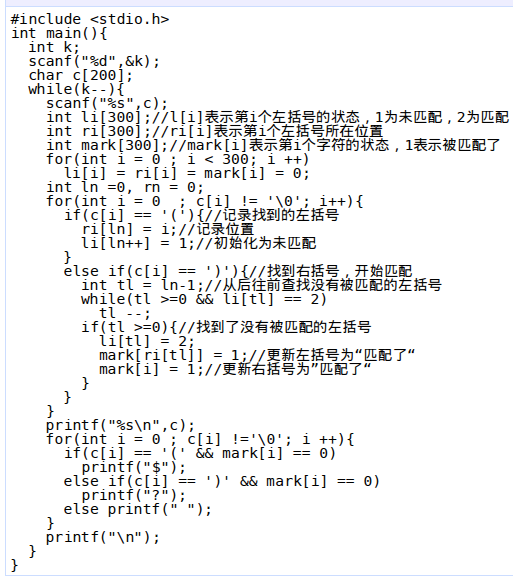
\includegraphics[width=0.9\hsize]{pic/扩号匹配问题-good.png}
     \end{columns}
     }
}

\subsection{7.连续整数区域上确界}
\frame{
  \frametitle{7.连续整数区域上确界}
  
     \only<1>{\centering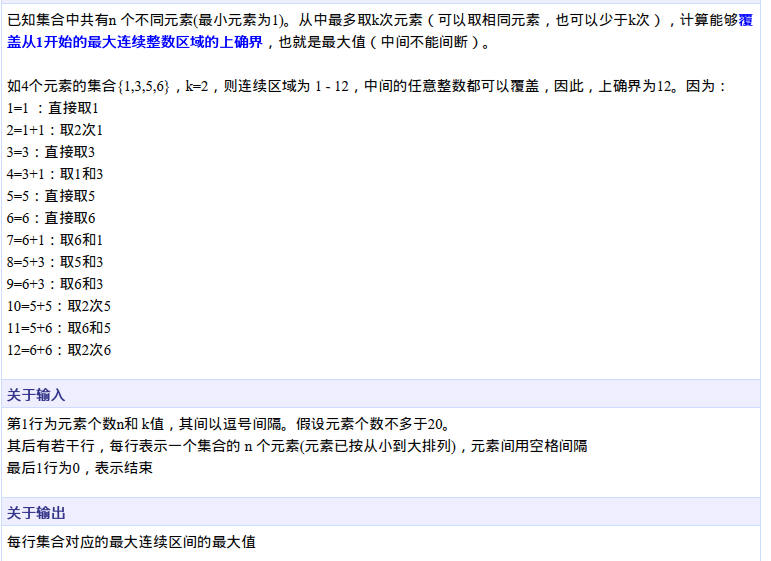
\includegraphics[width=0.9\hsize]{pic/连续整数区域上确界.png}}
     \only<2>{
     \begin{columns}
      \column{0.35\hsize}	
     \begin{itemize}
      \item 从sum=1开始,如果使用k次数组得不到和为sum,则停止
      \item 递归:至多使用k次等价于 至多使用k-1次得到和为sum-a[i]
     \end{itemize}
     
     \column{0.6\hsize}
     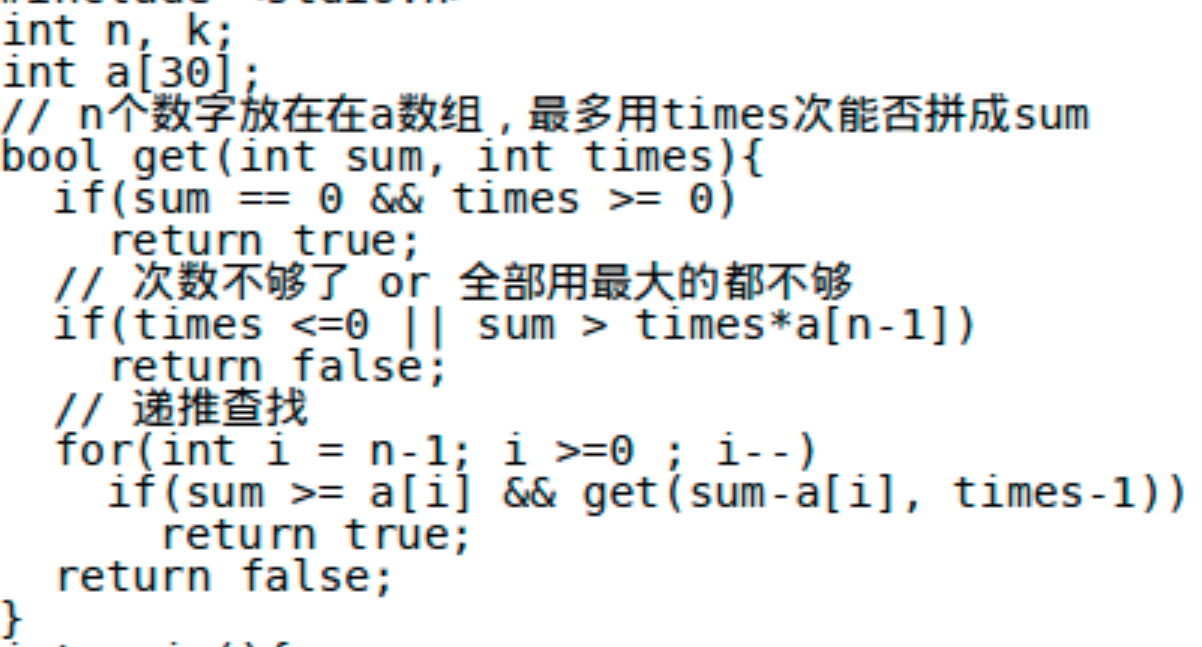
\includegraphics[width=0.9\hsize]{pic/连续整数区域上确界-good.png}
     \end{columns}
     }
}


\frame{
  \begin{columns}[c]
   \column{.15\hsize}
   \column{.7\hsize}
   \begin{block}{}
    \centering \Large 结构体与链表  \\ 
    \small --- 1207
   \end{block}
   \column{.15\hsize}
  \end{columns}
}


\subsection{1.删除数组中的元素(链表)}
\frame{
  \frametitle{1.删除数组中的元素(链表)}
  
     \only<1>{\centering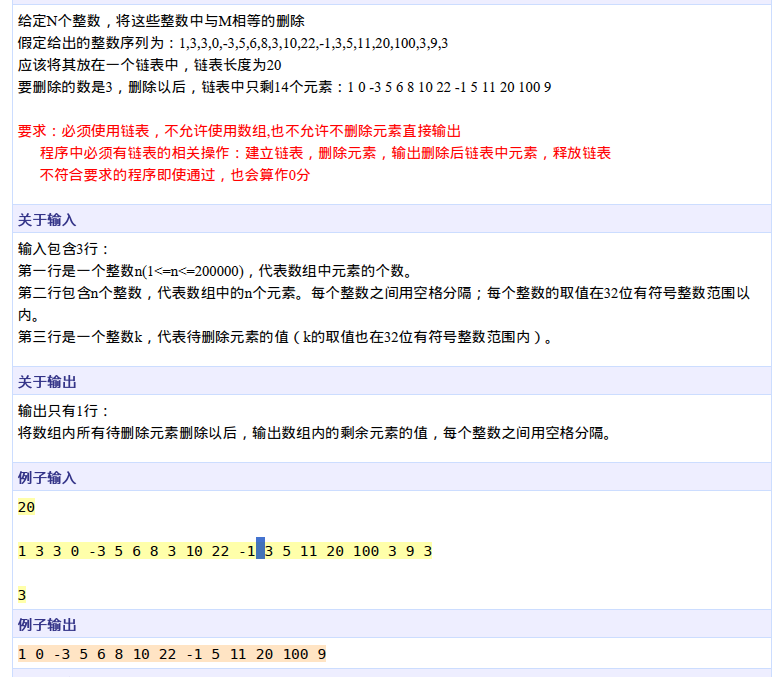
\includegraphics[width=0.75\hsize]{pic/删除数组中的元素(链表).png}}
     \only<2>{
     \begin{columns}
      \column{0.3\hsize}	
     \begin{itemize}
      \item 删除元素需要直到前一个元素
      \item 删除的是第一个元素呢?
     \end{itemize}
     \centering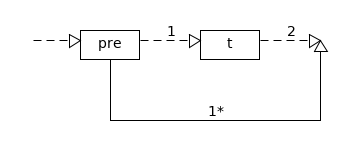
\includegraphics[width=0.9\hsize]{pic/删除链表元素.png}
     
     \column{0.7\hsize}
     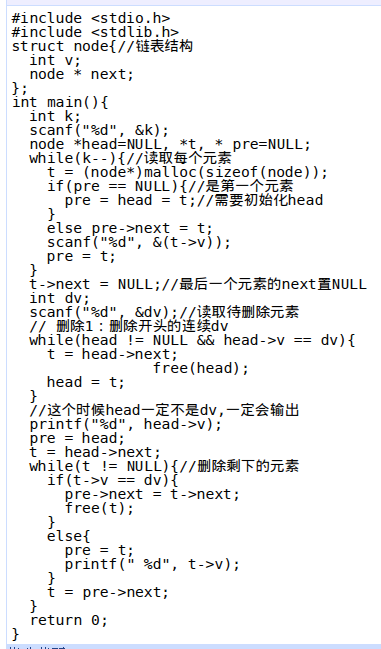
\includegraphics[width=0.6\hsize]{pic/删除数组中的元素(链表)-good.png}
     \end{columns}
     }
}


\frame{
  \frametitle{1.删除数组中的元素(链表)}
  
     \begin{columns}
      \column{0.3\hsize}	
      \large{我是怎么过的}
      \begin{enumerate}
       \item `Empty output file`没输出
       \only<3->{\item 还是没输出}
       \only<5->{\item 还是没输出}
       \only<7->{\item 还是没输出}
       \only<9->{\item 过了}
       
      \end{enumerate}

     \column{0.7\hsize}
     \only<1>{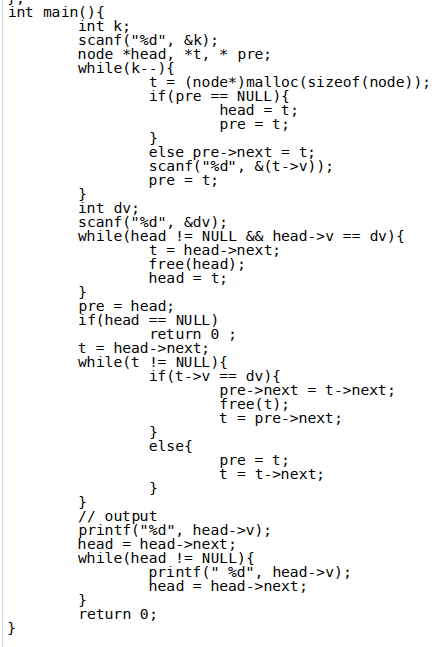
\includegraphics[width=0.6\hsize]{pic/删除1.png}}
     \only<2-3>{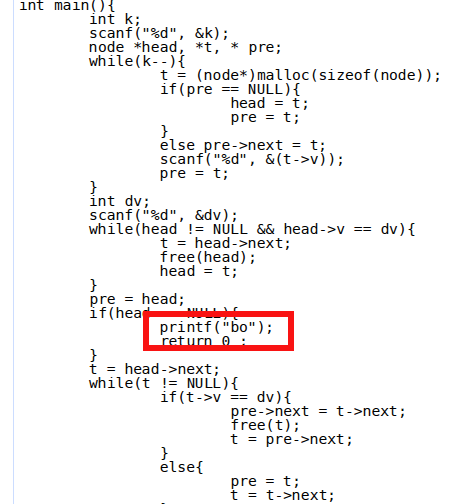
\includegraphics[width=0.6\hsize]{pic/删除2.png}}
     \only<4-5>{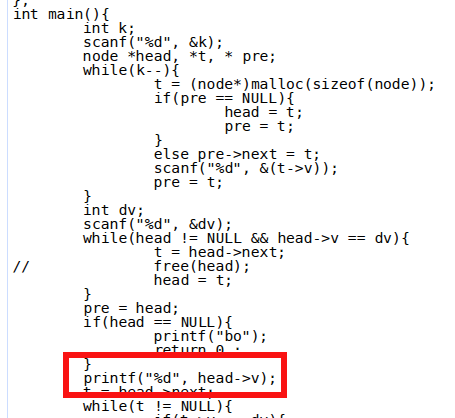
\includegraphics[width=0.6\hsize]{pic/删除3.png}}
     \only<6-7>{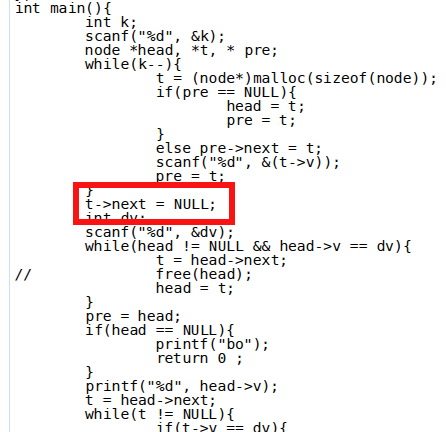
\includegraphics[width=0.6\hsize]{pic/删除4.png}}
     \only<8-9>{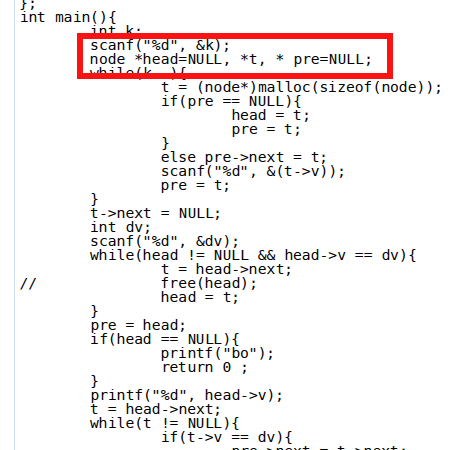
\includegraphics[width=0.7\hsize]{pic/删除5.png}}
     \end{columns}
}


\frame{
  \frametitle{2.统计学生信息(使用动态链表完成)}
  
     \only<1>{\centering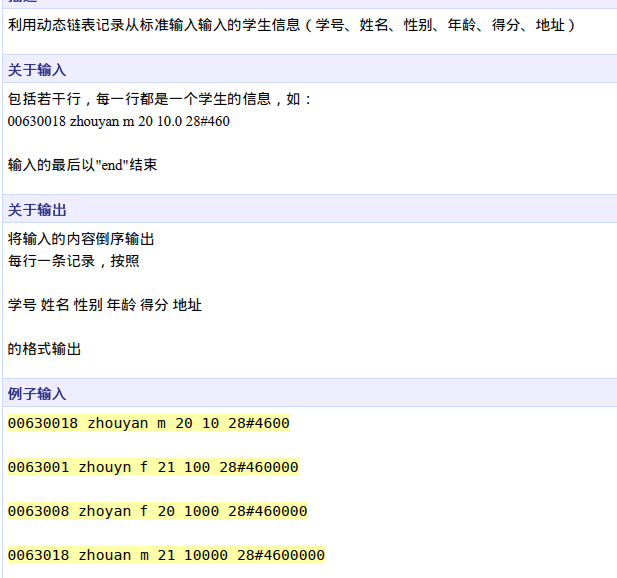
\includegraphics[width=0.75\hsize]{pic/统计学生信息(使用动态链表完成).png}}
     \only<2->{
     \begin{columns}
      \column{0.3\hsize}	
     \begin{itemize}\small
      \only<2>{\item 结构体,内部存每一行的信息和之前结构体的地址}
     \only<3->{
       \item \red{为什么我按每个元素读就又是`Empty output file`}
     }
     \only<4->{
       \item 打印第二组样例出来看一下?
     }
     \end{itemize}
     
     \column{0.7\hsize}
     \only<2>{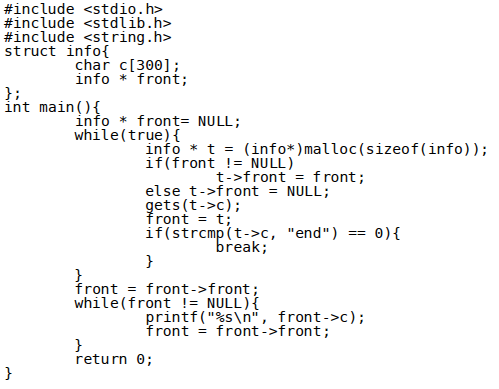
\includegraphics[width=0.9\hsize]{pic/统计学生信息.png}}
     \only<3>{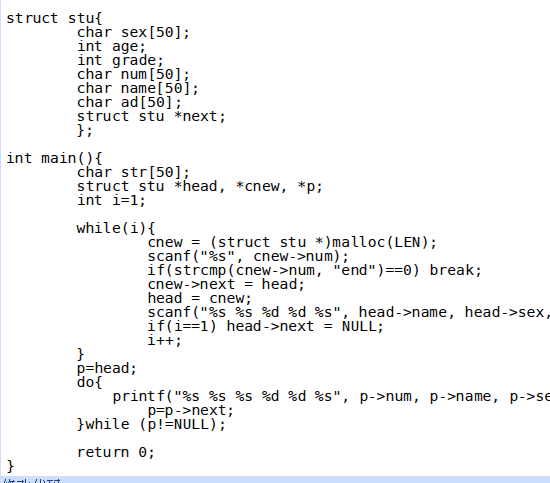
\includegraphics[width=0.9\hsize]{pic/统计学生信息(使用动态链表完成)-bad.png}}
     \only<4>{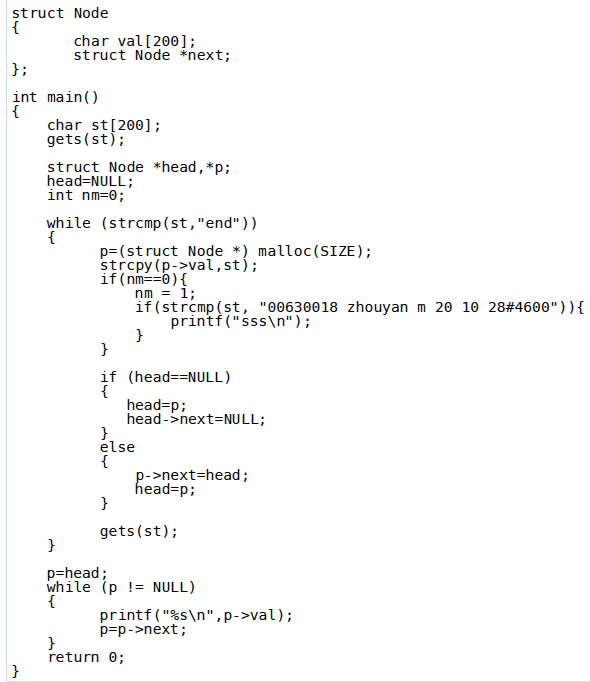
\includegraphics[width=0.8\hsize]{pic/统计学生信息(使用动态链表完成)-bad2.png}}
     \only<5>{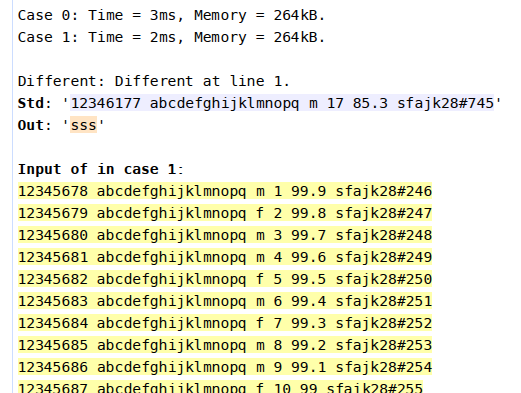
\includegraphics[width=0.9\hsize]{pic/统计学生信息(使用动态链表完成)-bad3.png}}
     \end{columns}
     }
}

\frame{
  \frametitle{3.谁拿了最多奖学金(不讲)}
     \only<1>{\centering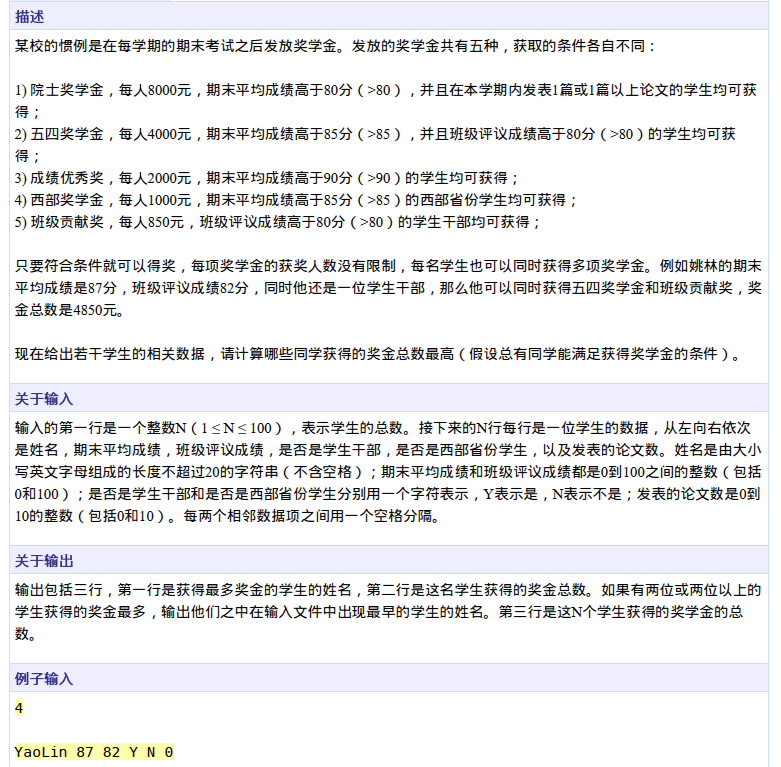
\includegraphics[width=0.65\hsize]{pic/谁拿了最多奖学金.png}}
     \only<2>{\centering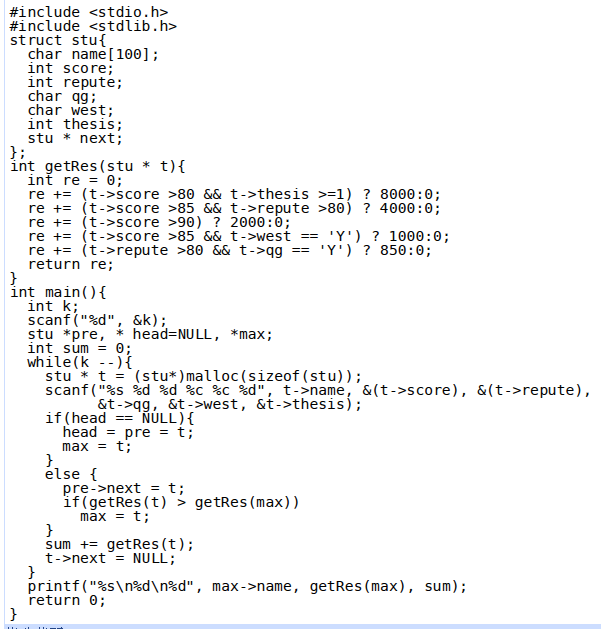
\includegraphics[width=0.65\hsize]{pic/谁拿了最多奖学金-good.png}}
}

\frame{
  \frametitle{4.班级学生成绩统分}
  
     \only<1>{\centering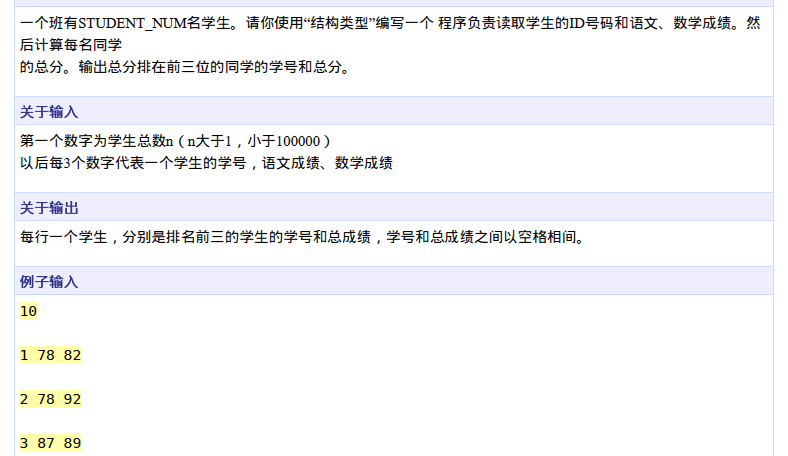
\includegraphics[width=0.75\hsize]{pic/班级学生成绩统分.png}}
     \only<2>{
     \begin{columns}
      \column{0.3\hsize}	
     \begin{itemize}
      \item 注意保序(等于时不替换)
      \item 排序一定会超时
     \end{itemize}
     
     \column{0.7\hsize}
     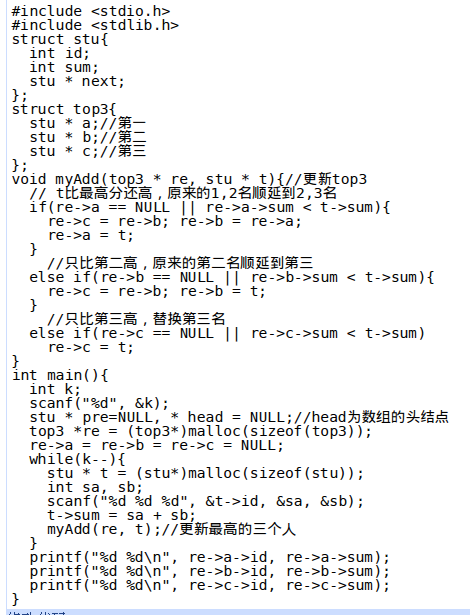
\includegraphics[width=0.6\hsize]{pic/班级学生成绩统分-good.png}
     \end{columns}
     }
}

\frame{
  \frametitle{5.链表合并排序}
  
     \only<1>{\centering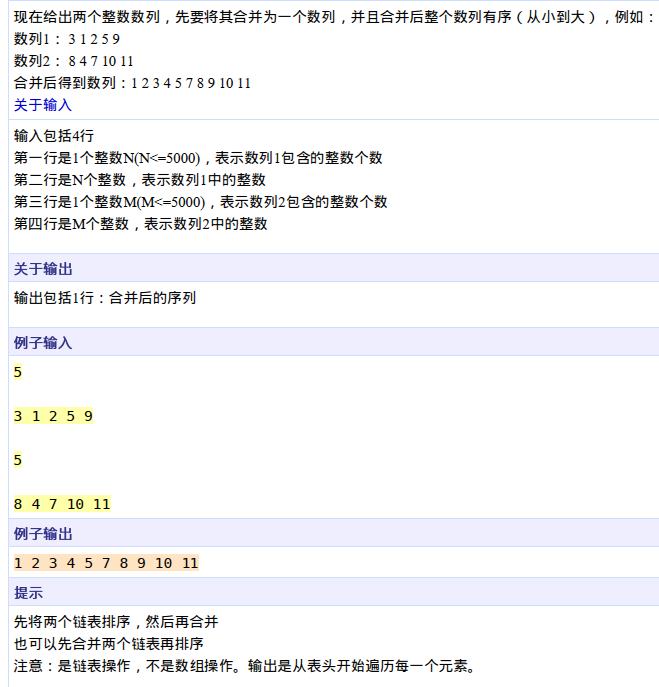
\includegraphics[width=0.6\hsize]{pic/链表合并排序.png}}
     \only<2>{
     \begin{columns}
      \column{0.3\hsize}	
     \begin{itemize}
      \item 先合并,再排序
      \\item 冒泡排序需要知道前一个节点
     \end{itemize}
     
     \column{0.7\hsize}
     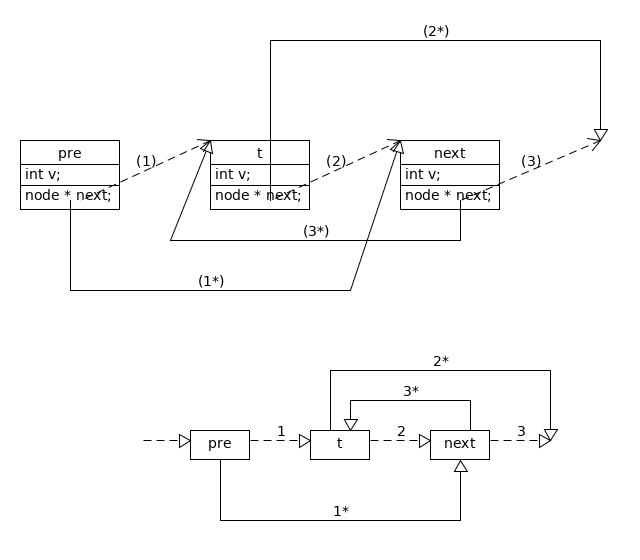
\includegraphics[width=0.9\hsize]{pic/交换位置.png}
     \end{columns}
     }
     \only<3>{
     \begin{columns}
      \column{0.3\hsize}	
     \begin{itemize}
      \item 给一种解法
     \end{itemize}
     
     \column{0.7\hsize}
     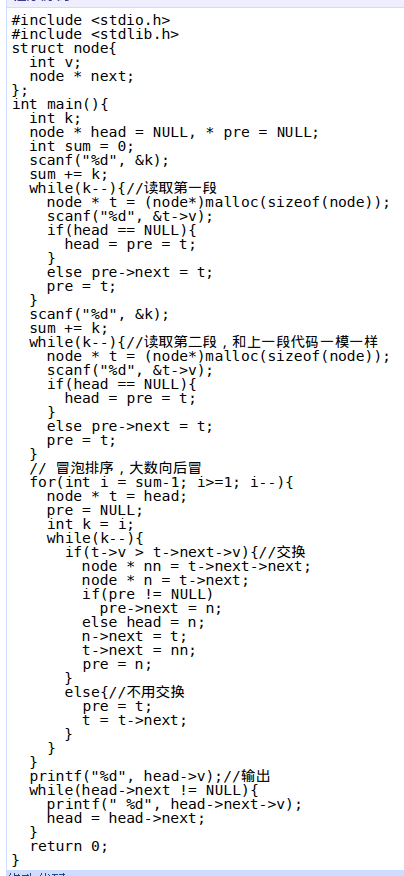
\includegraphics[width=0.45\hsize]{pic/链表合并排序-good.png}
     \end{columns}
     }
} 

\frame{
  \frametitle{5.链表合并排序}
  我是怎么调试的
  \begin{columns}
   \column{0.45\hsize}
     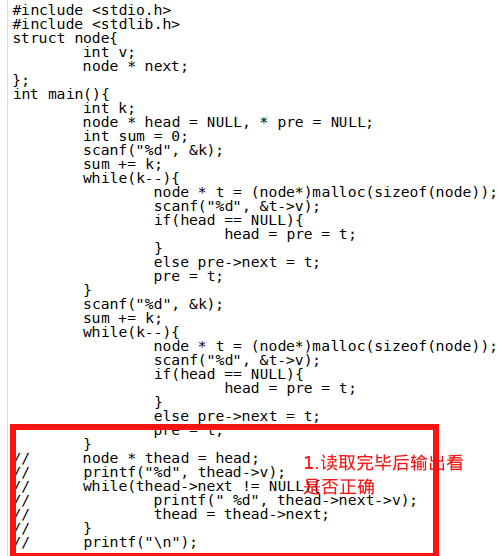
\includegraphics[width=0.95\hsize]{pic/debug1.png}
   \column{0.55\hsize}
     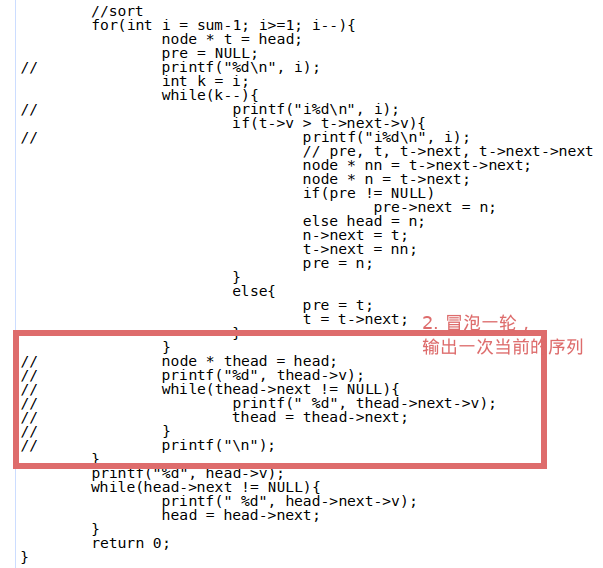
\includegraphics[width=1\hsize]{pic/debug2.png}
  \end{columns}

  
  
}


\frame{
  \begin{columns}[c]
   \column{.15\hsize}
   \column{.7\hsize}
   \begin{block}{}
    \centering \Large 综合练习  \\ 
    \small --- 1201
   \end{block}
   \column{.15\hsize}
  \end{columns}
}

\frame{
  \frametitle{1.旋转输出矩阵}
  
     \only<1>{\centering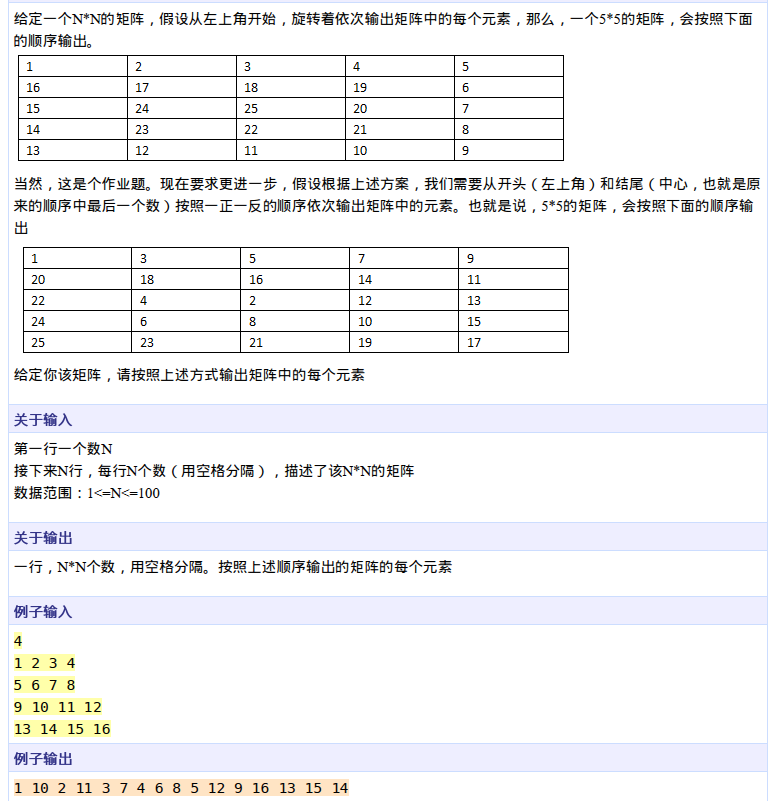
\includegraphics[width=0.65\hsize]{pic/旋转输出矩阵.png}}
     \only<2>{
     \begin{columns}
      \column{0.3\hsize}	
     \begin{itemize}
      \item 和上机模拟的`二维数组回形遍历`类似
      \item 先从一个方向把二维数组输出到一维数组中
      \item 再头尾两个指针输出(两端夹逼)
     \end{itemize}
     
     \column{0.7\hsize}
     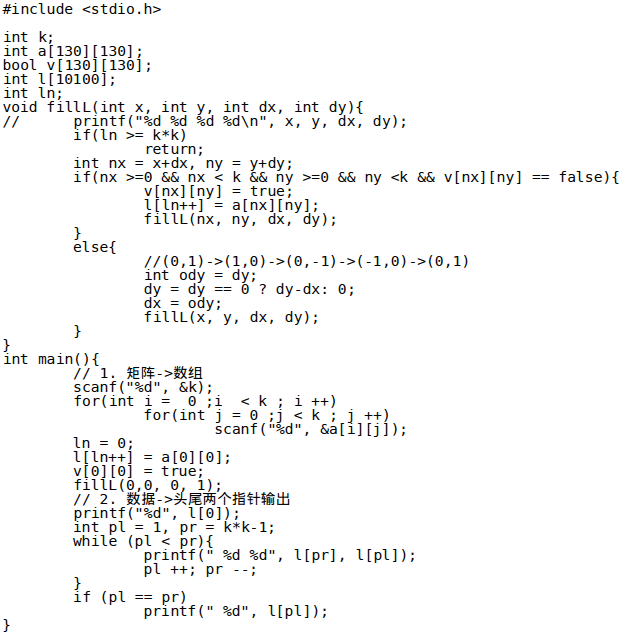
\includegraphics[width=0.85\hsize]{pic/旋转输出矩阵-good.png}
     \end{columns}
     }
}

\frame{
  \frametitle{2.不能一起吃的食物}
     \only<1>{\centering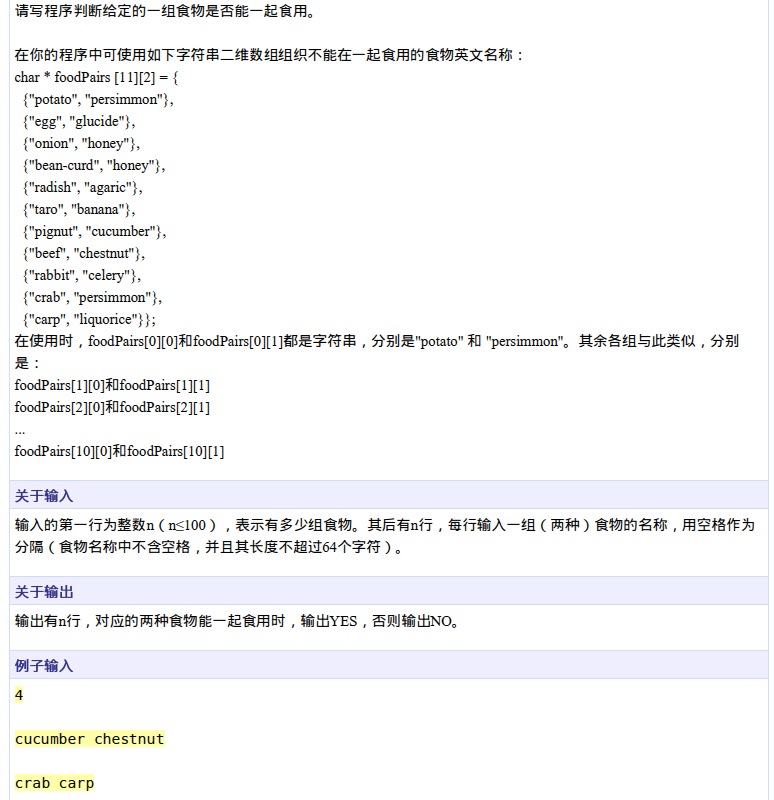
\includegraphics[width=0.65\hsize]{pic/不能一起吃的食物.png}}
     \only<2>{
     \begin{columns}
      \column{0.3\hsize}	
     \begin{itemize}
      \item 每次读取食物对,判断是否在已知的数组中,注意两种顺序都要考虑
      \item 不需要存储所有的食物对,可以读一对,输出一对
     \end{itemize}
     
     \column{0.7\hsize}
     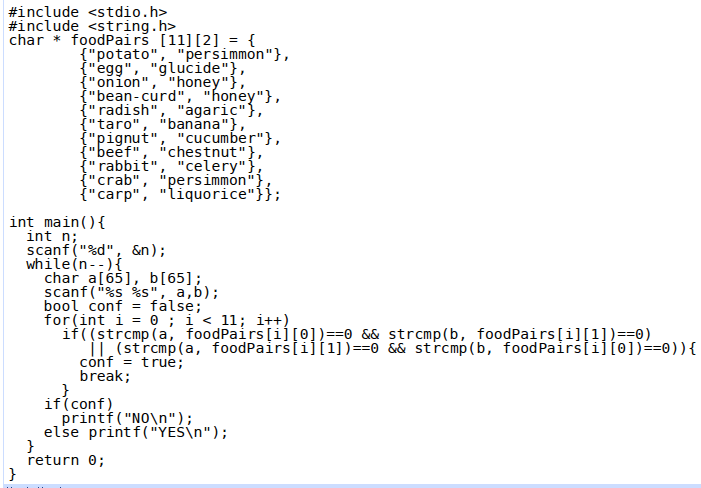
\includegraphics[width=0.85\hsize]{pic/不能一起吃的食物-good.png}
     \end{columns}
     }
  
}
\frame{
  \frametitle{3.算24}
     \only<1>{\centering\includegraphics[width=0.65\hsize]{pic/算24.png}}
     
      \only<2>{\begin{itemize}
                \item 有同学是这样过的
               \end{itemize}
      \includegraphics[width=0.85\hsize]{pic/算24-bad.png}}
      
     \only<3->{
     \begin{columns}
      \column{0.3\hsize}	
     \begin{itemize}\footnotesize
      \only<3>{
      \item 我把1500011105同学的代码注释了作为样例
      \item 递归,每次做一步运算,枚举每种情况
      \item 运算前保留原状态,运算结束后还原,为下一次运算做准备
      \item 理论上是近似解:和24的差值小于$10^{-9}$
     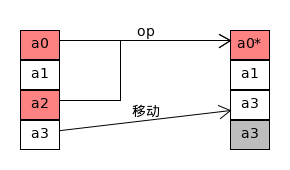
\includegraphics[width=0.85\hsize]{pic/算24-思路.png}}
      \only<4>{\item 再贴一个我过的样例,不是特别好
      \item 每个函数都被其下面紧邻的函数调用}
     \end{itemize}
     
     \column{0.7\hsize}
     \only<3>{\includegraphics[width=0.85\hsize]{pic/算24-good2.png}}
     \only<4>{\includegraphics[width=0.99\hsize]{pic/算24-good1.png}}
     \end{columns}
     }
}
\frame{
  \frametitle{4.进制转换}
  
     \only<1>{\centering\includegraphics[width=0.65\hsize]{pic/进制转换.png}}
     \only<2->{
     \begin{columns}
      \column{0.3\hsize}	
     \begin{itemize}
      \item 贴两个例子
      \item 先将14进制数转化成十进制,然后将十进制转换成7进制打印
     \end{itemize}
     
     \column{0.7\hsize}
     \only<2>{\includegraphics[width=0.85\hsize]{pic/进制转换-good1.png}}
     \only<3>{\includegraphics[width=0.85\hsize]{pic/进制转换-good2.png}}
     \end{columns}
     }
}

\frame{
  \frametitle{5.计算反序数(不讲)}
  
     \only<1>{\centering\includegraphics[width=0.65\hsize]{pic/计算反序数.png}}
     \only<2->{
     \begin{columns}
      \column{0.3\hsize}	
     \begin{itemize}
      \item 不讲了,直接贴代码
      \item 几个特殊情况(都包含在样例里了)

     \end{itemize}
     
     \column{0.7\hsize}
     \only<2>{\includegraphics[width=0.65\hsize]{pic/计算反序数-good.png}}
     \end{columns}
     }
}
\frame{
  \frametitle{6.放苹果问题(不讲)}
  
     \only<1>{\centering\includegraphics[width=0.65\hsize]{pic/放苹果问题.png}}
     \only<2->{
     \begin{columns}
      \column{0.3\hsize}	
     \begin{itemize}
      \item 递推式已经给出,方法见代码
     \end{itemize}
     
     \column{0.7\hsize}
     \only<2>{\includegraphics[width=0.85\hsize]{pic/放苹果问题-good.png}}
     \end{columns}
     }
}
\frame{
  \frametitle{7.奇数单增序列(不讲)}
  
     \only<1>{\centering\includegraphics[width=0.65\hsize]{pic/奇数单增序列.png}}
     \only<2->{
     \begin{columns}
      \column{0.3\hsize}	
     \begin{itemize}
      \item 方法见代码
     \end{itemize}
     
     \column{0.7\hsize}
     \only<2>{\includegraphics[width=0.75\hsize]{pic/奇数单增序列-good.png}}
     \end{columns}
     }
}	
\frame{
  \frametitle{8.因式分解}
  
     \only<1>{\centering\includegraphics[width=0.65\hsize]{pic/分解因数.png}}
     \only<2->{
     \begin{columns}
      \column{0.3\hsize}	
     \begin{itemize}
      \item 方法见代码
     \end{itemize}
     
     \column{0.7\hsize}
     \only<2>{\includegraphics[width=0.85\hsize]{pic/因式分解-good.png}}
     \end{columns}
     }
}	

\frame{
  \frametitle{9.前缀表达式}
  
     \only<1>{\centering\includegraphics[width=0.85\hsize]{pic/前缀表达式.png}}
     \only<2->{
     \begin{columns}
      \column{0.4\hsize}	
     \begin{itemize}\footnotesize
      \only<2>{\item 思路1:按照要求来:出现连续两个整数,就应该用他们加上他们之前的运算符进行运算,将三个元素替换成一个元素,然后不断做,直到只剩一个元素,就是我们要的结果}
      \only<3>{\item 思路2:递归
	\begin{itemize}\footnotesize
	 \item block = (+) (subBlock1) (subBlock2)
	 \item subBlock1 = (-) (subBlock11) (subBlock12)
	\end{itemize}
	}
     \end{itemize}
     
     \column{0.6\hsize}
     \only<2>{\includegraphics[width=0.85\hsize]{pic/前缀表达式-good.png}}
     \only<3>{\includegraphics[width=0.7\hsize]{pic/前缀表达式-good2.png}}
     \end{columns}
     }
}

\frame{
  \frametitle{10.文字排版(不讲)}
  
     \only<1>{\centering\includegraphics[width=0.65\hsize]{pic/文字排版.png}}
     \only<2->{
     \begin{columns}
      \column{0.3\hsize}	
     \begin{itemize}
      \item 直接放代码了
      \item 记录当前行的宽度$lineLen$,如果加上下一个单词之后长度大于80,则下一个单词要换行输出,并且新行的宽度变成下一个单词的长度
     \end{itemize}
     
     \column{0.7\hsize}
     \only<2>{\includegraphics[width=0.85\hsize]{pic/文字排版-good.png}}
     \end{columns}
     }
}
\frame{
  \frametitle{11.验证子串(不讲)}
  
     \only<1>{\centering\includegraphics[width=0.65\hsize]{pic/验证子串.png}}
     \only<2->{
     \begin{columns}
      \column{0.3\hsize}	
     \begin{itemize}
      \item 直接放代码了
      \item $strstr(s1,s2)$返回s2在s1中作为子串出现是的首地址
     \end{itemize}
     
     \column{0.7\hsize}
     \only<2>{\includegraphics[width=0.85\hsize]{pic/验证子串-good.png}}
     \end{columns}
     }
}

\frame{
  \frametitle{几个问题/建议}
  \begin{itemize}
   \item 想好怎么做(过程)再写代码
   \item 提高=读懂别人的代码+\red{\textbf{自己实现}}
   \item 常用函数的头文件背好
   \item 本地运行过不了样例的,提交上去99.999999999\%过不了
   \item 很奇怪的数/字符(-1208899956,烫烫烫):数组越界!
   \item `Empty output file`没输出:\red{数据没读完(程序没有足够的内存记录待读入的数据)} 或者 程序中有死循环
   \item $int num[300] = \{0\}$的含义:只初始化$nums[0]=0$,之后的数据值\red{未知}
  \end{itemize}
  
}

\frame{
  \frametitle{最后}
  
  \begin{columns}\centering
   \column{0.5\hsize}
   \includegraphics[width=0.85\hsize]{pic/anny.jpg}
   \column{0.5\hsize}
   \includegraphics[width=0.85\hsize]{pic/anny-origin.jpg}
  \end{columns}

}

\end{document} 